\numberwithin{equation}{section}

\externaldocument{chapter1}

\chapter{Congruence subgroups of $\sltz$}

\section{The principal congruence subgroup $\Gamma(N)$}
Recall the notation $\sltz = \Gamma$. 
\begin{definition} The group denoted $\Gamma(N)$,  $N \in \mathbb{N^+}$, is called the principal congruence subgroup of level $N$, defined to be
$$\Gamma(N) := \Big  \lbrace  A= \left(\begin{array}{ c c } a & b \\ c & d \end{array} \right) \in \Gamma \, \Big \vert \, A \equiv   \left(\begin{array}{ c c } 1 & 0 \\ 0 & 1 \end{array} \right) \mod N \Big  \rbrace$$
We define $\Gamma(1)  := \Gamma$.
\end{definition}
This subgroup $\Gamma(N)$ is actually a normal subgroup in $\Gamma$ since it is the kernel of the group homomorphism from $\sltz \rightarrow \sltznz$ obtained by reducing entries modulo $N$. Notice that $a \equiv x \mod Nt \implies a \equiv x \mod N$ so for any multiple $Nt$ we get $\Gamma(Nt) \subset \Gamma(N)$.
\\
We will make use of the following elementary lemma in several proofs.
\begin{lemma}\label{lem:elementaryCoprime}
Given integers $c \neq 0,\, d,\, N  \in \mathbb{Z}$. The set $\{t \, \vert \, (d + tN, c) = 1 \}$ is non-empty, and this set is infinite if there exists a prime dividing $c$ but not $d$. (I.e $\gcd(c,d) \neq c \text{ or }  d$).
\end{lemma}
\begin{proof}
Let $d' = d+ tN$. Our goal is to find appropriate values for $t$.
\\ 
We begin by splitting the prime divisors of $c$ into two groups, 
\\ 
$$\{p_1,p_2,\dots,p_s \colon \, p_i \mid c \,,\, p_i \mid d\} \text{ and } \{q_1,q_2,\dots, q_r \colon q_j \mid c\, ,\, q_j \nmid d\}$$

If $\gcd(c,d) \neq c \text{ or } d$ : then the set of $q_j$ is non empty.\\
Define $k = \prod{q_j} = \prod_{p\mid c,p\nmid d}p$, and $d' = d + tN$, where $t = k^m$. Where $m$ any positive integer.\\
Suppose $p$ is a prime divisor of $c$ and $d'$. \\
Suppose also $p \mid d$, then $p \mid (d' -d)  = tN$ and $p \nmid t$. This implies $p \mid N$, which is a contradiction, since $\gcd(c,dN) =1$. \\
Otherwise if $p \nmid d$, then $p \nmid (d' -d) = tN$ and $p \mid t$. These two results contradict.  \\
So there are no common prime divisors of $c,d'$ and so $gcd(c,d' = d + k^m) = 1$, for all $m \in \mathbb{N}$.\\
\\
In the other case, if $\gcd(c,d) = c \text{ or } d$, define $d' = d+ N$. Now $\gcd(c,d') =1$ since $\gcd(c,d,N) =1$.
\end{proof}

\begin{theorem}\label{thm:surjective}
The natural map $\sltz \rightarrow \sltznz$ is surjective.
\end{theorem}

\begin{proof}
Let $\gamma = \left( \begin{array}{ c c } \bar{a} & \bar{b}  \\ \bar{c} & \bar{d} \end{array} \right) \in \sltznz$ be given. A lift of $A \in \sltznz$ to  $M_2(\mathbb{Z})$ is an element in the inverse image of $A$ by the reduction homomorphism. Let $\tilde{\gamma} = \left(
  \begin{array}{ c c }
     a & b \\
     c & d
  \end{array} \right) \in M_2(\mathbb{Z})$, such that $\tilde{\gamma} \equiv \gamma \mod N$.
We show it's possible to modify $\tilde{\gamma}$ such that it's still congruent to $\gamma$ but has unit determinant.\\
\\
First note that $ad -bc \equiv 1 \mod N$. So $ad - bc +Nk = 1$ for some $k \in \mathbb{Z}$, so $\gcd(c,d,N) = 1$.\\
We suppose $c \neq 0$ for now. We can apply Lemma \ref{lem:elementaryCoprime} to find a $d'$ such that $\gcd(c,d') =1$, and $d' \equiv d \mod N$. Define $\tilde{\gamma_1} = \left( \begin{array}{ c c } a & b \\ c & d' \end{array} \right) \equiv \gamma$.\\
We can now consider lifts of $\gamma$ of form $ \tilde{\gamma_2} = \left(
    \begin{array}{cc}
        a+kN & b+lN  \\
        c    & d'
    \end{array} \right)$, $k,l \in \mathbb{Z}$. The determinant is $\det(\tilde{\gamma_2}) = (a+kN)d' - (b+lN)c = ad' - bc +N(kd'-lc)$.\\  From the definition of $\gamma_1$ we have $ad' - bc = 1 + qN$ for some $q\in \mathbb{Z}$. By substitution, $\det(\tilde{\gamma_2}) = 1 + N(q + kd' - lc) = 1$.\\
Now the fact that $\gcd(c,d') = 1$ allows us to solve $q = lc - kd'$ for $k,l 
\in \mathbb{Z}$. We obtain the lift,
$$\left(
    \begin{array}{cc}
        a +kN & b +lN  \\
        c    & d'
    \end{array} \right) \in \sltz \equiv \gamma \mod N$$
The case $c = 0$ is not much different. The condition $\det(\gamma) =1$ gives that $d \neq 0$, and we proceed similarly to above. We have $\gcd(a,d,N) =1$, and we set $d' = d + tN$ where $t = \prod_{p\mid a,p\nmid d}p$. This gives $gcd(d',a) =1$. Then we compute $q$ from $ad = 1+qN$. Finally we solve $ax + yd' = -q$ for integers $x, \,y$. Our desired lift is then $\left(
    \begin{array}{cc}
        a+yN & b  \\
        0    & d' + xN
    \end{array} \right)$
\end{proof}


\begin{theorem} \label{thm:-IT2U2genGamma2}
The group $\Gamma(2)$ is generated by the matrices $-I,T^2$ and $U^2$, where $T = \tm,U = \um$ as before, so $T^2 = \left(\begin{array}{ c c } 1 & 2 \\ 0 & 1 \end{array} \right)$ and $U^2 = \left(\begin{array}{ c c } 1 & 0 \\ 2 & 1 \end{array} \right)$. 
\end{theorem}
\begin{proof}
We have that $-I,T^2,U^2 \in \Gamma(2)$  so $\langle -I,T^2,U^2 \rangle \subset \Gamma(2)$. For the reverse inclusion we adapt the algebraic proof that $\langle S,T\rangle = \sltz$. We will use the modified division theorem, that is, given $a,b \in \mathbb{Z}$ we can write $a = bq + r$ where $ |r| \leq |b|/2$.\\
So we pick any $A  =  \left(\begin{array}{ c c } a & b \\ c & d \end{array} \right) \in \Gamma(2)$, the definition gives that $a,d$ are odd and $b,c$ are even. \\
If $c=0$, then $ad-bc = ad = 1$ implies that $a=d = \pm 1$, also $b$ is even so can write as $b = 2k$ so $A =  \left(\begin{array}{ c c } \pm 1 & 2k \\ 0 & \pm 1 \end{array} \right) \in \Gamma(2)$. This is of the form $ \pm T^{2k} = \pm {T^2}^k \in \langle -I, T^2 \rangle$.\\
What we wish to show is that every matrix in $\Gamma(2)$ can be reduced to a matrix with lower left entry 0 by an element of $-I,T^2,U^2$.
We can proceed by induction on the size of $c$, the lower left entry. If $c=0$ we are done by the above.\\
Suppose every matrix in $\Gamma(2)$ with lower left entry,$c$ , such that $|c| < n$, can be reduced to a matrix with lower left entry 0 by an element of $-I,T^2,U^2$. \\
Now suppose we have a matrix $\left(\begin{array}{ c c } a & b \\ c & d \end{array} \right) \in \Gamma(2) $ with $ |c| = n$. From the definition of $\Gamma(2)$ we see that $a$ and $c$ have different parity, so $|a| \neq |c|$, there are two possibilities.
If $|a| < |c|$, use the modified division theorem to write $c = (2a)q + r$, where $|r| \leq |2a|/2 =|a|$. Then 
$$U^{-2q}A =  \left(\begin{array}{ c c } 1 & 0 \\ -2 & 1 \end{array} \right)\left(\begin{array}{ c c } a & b \\ c & d \end{array} \right) = \left(\begin{array}{ c c } a & b \\ c-2qa & d-2qb \end{array} \right) = \left(\begin{array}{ c c } a & b \\ r & d-2qb \end{array} \right)$$.
Now the matrix $U^{-2q}A$ has lower left entry $r$, and $|r| < |c|$, i.e lower left entry less in absolute value than before, so we can conclude by the induction hypothesis.
If $|a| > |c|$, then use the modified division theorem to write $a = (2c)q + r$, where $|r| \leq |2c|/2 = |c|$. Then 
$$T^{-2q}A = \left(\begin{array}{ c c } 1 & -2 \\ 0 & 1 \end{array} \right)\left(\begin{array}{ c c } a & b \\ c & d \end{array} \right) =  \left(\begin{array}{ c c } a-2qc & b-2qd \\ c & d \end{array} \right) = \left(\begin{array}{ c c } r & b-2qd \\ c & d \end{array} \right)$$ 
Now the upper left entry $r$ is less in absolute value than the lower left entry so we can apply the first case and then conclude by induction.
\\
This shows we can find $g \in  \langle -I, T^2, U^2 \rangle$, such that $gA$ has lower left entry 0. This is of the form $gA = \pm T^{2k} \in \langle -I, T^2 \rangle \implies A = \pm g^{-1} T^{2k} \in \langle -I, T^2, U^2 \rangle$.

\end{proof}




\begin{lemma}\label{lem:orderofslznzpe}
The order of $\sltznz[p^e] $ is $p^{3e}( 1- 1/p^2)$ when $p$ is prime and $e \in \mathbb{N}$. 
\end{lemma}
\begin{proof}
 The case $e=1$ can be computed by considering two subcases and counting the number of possible $A =  \left(\begin{array}{ c c }  a& b \\ c & d \end{array} \right) \in \sltznz[p] $. The definition of $\sltznz[p]  $ gives us that $A \in \sltznz[p]  $ if and only if $ det(A) = ad -bc \equiv 1 \mod p$. The number of solutions to this equation in $\mathbb{Z}/p\mathbb{Z}$ is equal to the number of possible $A$. A key fact we will use is that $(\mathbb{Z}/p\mathbb{Z})^* = \znz[p] \setminus \{\bar{0}\}$, so each non-zero element in $\znz$ has a unique multiplicative inverse ($\star$).\\
 
    Case $a\equiv0$ : $A =  \left(\begin{array}{ c c }  0 & b \\ c & d \end{array} \right)$, and $\det(A) = -bc \equiv 1\mod p$. We can apply $(\star)$ to say there are $p-1$ solutions in $b,c$ to this congruence. Also $d$ can take any of $p$ values in $\znz$. The total gives $p\cdot(p-1) = p(p-1)$ solutions to $ad -bc \equiv 1 \mod p$ for $a \equiv 0,b,c,d  \in \znz[p]$. \\
    
    Case $a\not \equiv 0$ : We can rearrange the equation to $ad \equiv 1+bc \mod p$. There are $p-1$ possible values for $a \not \equiv 0$, and $p$ possible values for each $b$ and $c$. From these the value for $d$ is determined uniquely by $(\star)$. In total there are $(p-1)\cdot p \cdot p \cdot 1 = (p-1)p^2$ in solutions to $ad -bc \equiv 1 \mod p$ for $a \not \equiv 0, b,c,d \in \znz[p]$.
\\    
    Totaling from both cases we have $p(p-1) + (p-1)p^2 = p^3 - p$ solutions to the equation for determinant. So the order of $\sltznz[p]$  is $p^3 - p$.\\
    The case  $e>1$ is more complex since then for $a\not\equiv 0$ the relation $ad \equiv 1+bc \mod p^e$ is not always solvable so we would have to separately consider further subcases $a$ invertible and not invertible $\mod p$. \\ 
We can proceed by induction on $e$.  We have shown $\sltznz[p^e] \vert = p^{3e}(1 - 1/p^2)$ for $e =1$. \\
Suppose that the result holds for $e = k$, i.e
$$\vert \sltznz[p^k] \vert = p^{3k}(1 - 1/p^2).$$ 
Consider the reduction homomorphism 
$$f: \sltznz[p^{k+1}] \to \sltznz[p^k] $$
$$f(\left(\begin{array}{ c c }  a& b \\ c & d \end{array} \right) = \left(\begin{array}{ c c }  a & b \\ c & d \end{array} \right) \mod p^k$$
The kernel of $f$ is, $$\Big \lbrace A \in \sltznz[p^{k+1}]  \Big \vert A = \left(
      \begin{array}{ c c }
         1+a'p^k & b'p^k \\
         c'p^k &  1+d'p^k 
      \end{array} \right) \text{ and } 0 \leq a',b',c',d' < p \in \mathbb{Z}/p^{k+1}\mathbb{Z} \Big \rbrace $$
Again we can count the number of possible matrices by counting the number of solutions to the determinant equation.
\begin{align*}
A\in ker(f) &\iff \det(A) \equiv 1 \mod p^{k+1}\\
			 & \iff  ( 1+a'p^k)( 1+d'p^k ) - (b'p^k)(c'p^k) \equiv 1 \mod p^{k+1}\\
             & \iff  1 + a'p^k + d'p^k + a'd'p^{2k} - b'c'p^k \equiv 1 \mod p^{k+1}\\
             & \iff   a'p^k + d'p^k  \equiv 0\mod p^{k+1}\\
             & \iff a' \equiv -d' \mod p
\end{align*}
So we if we let $d' = np -a'$ for some $n \in \znz[p]$, we can rewrite,
\begin{align*}
\lbrace A \in \sltznz[p^{k+1}]  \Big \vert A = \left(
      \begin{array}{ c c }
         1+a'p^k & b'p^k \\
         c'p^k &  1+(np- a')p^k 
      \end{array} \right) \\
       \text{ and } 0 \leq a',b',c', (np -a') < p\,, n\, \in \mathbb{Z}/p^{k+1}\mathbb{Z} \Big \rbrace
\end{align*}  
The restriction $0\leq a',(np - a') < p$ means we must have $n =1$. A matrix in $ker(f)$ is thus determined uniquely by the values $0 \leq a',b',c' < p$. The order of $ker(f)$ is thus the product of the number of possibilities for each value, ie $ker(f) = p^3$.\\ 
The reduction map $f$ is also surjective, this is because the reduction map from $\sltz \rightarrow \sltznz[p^k] $ is surjective and it can be decomposed into two maps $\sltz \rightarrow \sltznz[p^{k+1}]   \overset{f}{\rightarrow} \sltznz[p^k] $, so both the intermediate maps must be surjective.\\ 
We can apply the first isomorphism theorem to obtain $\sltznz[p^{k+1}] /ker(f) \cong \sltznz[p^k] $, and so
$$\vert \sltznz[p^{k+1}] \vert  = p^3 \vert \sltznz[p^k] \vert  \stackrel{\text{induction}}{=} p^{3(k+1)}(1 - 1/p^2)$$
\end{proof}

\begin{proposition} \label{prop:chineseRemainderTheorem}
Let $N\in \mathbb{Z}$, then, 
$$ \sltznz \cong \prod_{i=1}^k \sltznz[p_{i}^{r_i}]$$
Where $N = p_{1}^{r_1}\cdot\dots\cdot p_{k}^{r_k}$ is the prime factorization.
\end{proposition}
\begin{proof}
If we write $N$ as it's prime factorization $N = p_{1}^{r_1}
    \cdot\dots\cdot p_{k}^{r_k}$.
Define the homomorphism,
    $$f \, : \, \sltznz \to \prod_{i=1}^k \sltznz[p_{i}^{r_i}]$$
    $$\left(
      \begin{array}{ c c }
         a & b \\
         c & d
      \end{array} \right) \mapsto \Big( \left(
      \begin{array}{ c c }
         a & b \\
         c & d
      \end{array} \right) \mod p_{1}^{r_1} ,\dots, \left( \begin{array}{ c c }
         a & b \\
         c & d
      \end{array} \right) \mod p_{k}^{r_k} \Big)$$
      The function $f$ is well-defined, let $x\in \mathbb{Z}$, 
\begin{eqnarray*}
x \equiv x' \mod N \iff  N \mid (x-x') & \iff  & p_{1}^{r_1} \dots p_{k}^{r_k} \mid (x-x') \\
& \implies & p_i^{r_i} \mid (x-x') \iff x \equiv x' \mod  p_i^{r_i}
\end{eqnarray*}
\\
      To show $f$ is surjective, suppose we have  $\Big( \left(
      \begin{array}{ c c }
         a_1 & b_1 \\
         c_1 & d_1
      \end{array} \right) \in \sltznz[p_{1}^{r_1}],\dots, \left( \begin{array}{ c c }
         a_k & b_k \\
         c_k & d_k
      \end{array} \right) \in \sltznz[p_{k}^{r_k}]  \Big)$ 
      then we can find a matrix $A = \abcd \in M_2(\znz)$ by solving the corresponding system of congruences for each entry using the Chinese Remainder Theorem. For example, we take $a$ as the solution to the system \big($a \equiv a_1 \mod p_1^{r_1}\, ,\dots,a \equiv a_k \mod p_k^{r_k}$\big). We also must check $A$ does indeed lie in $\sltznz$, i.e $\det(A) \equiv 1 \mod N$. 
\\ 
For each $\left(\begin{array}{ c c }
         a_i & b_i \\
         c_i & d_i
      \end{array} \right) \in \sltznz[p_{i}^{r_i}]$ we have $a_i d_i - b_i c_i \equiv 1 \mod p_{i}^{r_i}$. Then $ad -bc \equiv 1 \mod p_{i}^{r_i}$ by definition of $a,b,c,d$. From this we see $p_{i}^{r_i} \mid (ad -bc ) -1$ for each prime power $p_{i}^{r_i}$, it follows that $ N = \prod_{i=1}^k p_{i}^{r_i} \mid (ad -bc) -1$. So $ ad -bc \equiv 1 \mod N$ and $A \in \sltz$.
\\
      To show injectivity suppose,
      $$f\big( \left(
      \begin{array}{ c c }
         a & b \\
         c & d
      \end{array} \right) \big) = f\big( \left(
      \begin{array}{ c c }
         a' & b' \\
         c' & d'
      \end{array} \right) \big)$$
      Then $a \equiv a' \mod p_i^{r_i}$ so by the Chinese Remainder Theorem $a \equiv a' \mod  p_{1}^{r_1} \dots p_{k}^{r_k} = N$, similarly we get $b\equiv b' \mod $, $c\equiv c' \mod N$,$d\equiv d' \mod N$.
\end{proof}


\begin{corollary} \label{cor:ordersltznz}
The order of $\sltznz$ is $N^3\prod_{p \mid N}(1 - 1/p^2)$.
\end{corollary}

\begin{proof}
From Proposition \ref{prop:chineseRemainderTheorem} we have $ \sltznz \cong \prod_{i=1}^k \sltznz[p_{i}^{r_i}]$.
So $$\vert \sltznz \vert = \prod_{p^e \mid N}\vert \sltznz[p^e]\vert = \prod_{p^e \mid N}p^{3e}(1 - 1/p^2)  = N^3\prod_{p \mid N}(1 - 1/p^2) $$
\end{proof}


\begin{corollary}\label{cor:generateordern}
The finite group $\sltznz$ is generated by two elements of order $N$. 
\end{corollary}

\begin{proof}
Every element of $\sltznz$ has a lift in $\sltz$. In Corollary \ref{cor:genInfiniteOrderUT} we showed $\langle T, U \rangle = \sltz$, where $T = \left(\begin{array}{ c c }  0& 1 \\ 1 & 1 \end{array} \right)\,,\, U = \left(\begin{array}{ c c }  1& 1 \\ 0 & 1 \end{array} \right)$. So this lift can be written as an element of $\langle T, U \rangle$. So reducing the lift modulo $N$ we get it as a product $T,U$ modulo $N$, i.e 
$$\sltznz = \langle \, T \mod N, U \mod N \, \rangle.$$ 
Also $T^n = \tm[n], U^n = \um[n]$ for all $n \in \mathbb{Z}$, so both have order $N$.
\end{proof}


\begin{corollary}\label{cor:reductionIsomorphism}
For any integer $N > 1$, 
$$\sltznz \cong \sltz / \Gamma(N) \text{ and } [\Gamma \, : \,  \Gamma(N)] =  N^3  \prod_{p\mid N}(1 - 1/p^2)$$
\end{corollary}

\begin{proof}
We have shown in Theorem \ref{thm:surjective} that the natural reduction map $\sltz \rightarrow \sltznz$ is onto and has kernel $\Gamma(N)$. The result follows from the first isomorphism theorem for groups. The index of $\Gamma(N)$ is exactly the order of $\sltznz$ which was computed Corollary \ref{cor:ordersltznz}.
\end{proof}
\section{General congruence subgroups}
We can define a more general notion of congruence subgroup than $\Gamma(n)$.
\begin{definition}
A subgroup of $\Gamma$ is called a congruence subgroup of level $N$ if it contains $\Gamma(N)$ and $N$ is the least such integer.
\end{definition}
The isomorphism in Corollary \ref{cor:reductionIsomorphism} is central to the study of congruence subgroups. It allows us to carry over properties of $\sltznz$ to $\sltz$ and vice versa. In particular we use the Third Isomorphism Theorem and the Correspondence Theorem in group theory to do so.


\begin{corollary}\label{cor:index3}
In $\sltz$ the subgroup $\langle S, T^2 \rangle$ has index $3$.
\end{corollary}

\begin{proof}
We begin by showing that $\Gamma(2) \subset \langle S, T^2 \rangle$. It is enough to show the generators $-I_2,T^2,U^2$ from theorem \ref{thm:-IT2U2genGamma2} are each in $\langle S, T^2 \rangle$. We have $-I_2 = S^2, T^2 = T^2$ and $ U^2 = ST^{-2}S^{-1}$. Now because $\Gamma(2)$ is a normal subgroup, when computing the index of $\langle S, T^2 \rangle$ it is equivalent to work modulo $\Gamma(2)$, i.e $[\sltz : \langle S, T^2 \rangle] = [\sltz / \Gamma(2) : \langle S, T^2 \rangle  / \Gamma(2)]$. This follows from the correspondence theorem. \\
The image of $\langle S, T^2 \rangle$ in $\sltz / \Gamma(2) \cong \sltznz[2] $ is $\{ \bar{I}, \bar{S} \}$, so $\langle S, T^2 \rangle  / \Gamma(2) \cong \{ \bar{I}, \bar{S} \}$. So finally we get
$$ [\sltz : \langle S, T^2 \rangle] = [\sltz / \Gamma(2) : \langle S, T^2 \rangle  / \Gamma(2)] = [ \sltznz[2]) : \{\bar{I}, \bar{S} \}] = 6/2 = 3 $$
\end{proof}

If we replace $\langle S , T^2 \rangle$ with $\langle S, T^m \rangle$ for $m >2$ there is no analog of corollary \ref{cor:index3} since $\langle S, T^m \rangle$ does not have finite index in $\sltz$ for $m >2$. The proof is omitted here but it sketched out in Conrad's expository paper on $\sltz$ \citep{conrad}.
\\
\\
The meaning of the terminology \textit{congruence} subgroup is that they can be described by a finite set of congruence conditions.

\begin{example}
It was shown in the proof of \ref{cor:index3} that $\Gamma(2) \subset \langle S, T^2 \rangle$ so $\langle S, T^2 \rangle$ is a congruence subgroup of level 2. We also showed that $\langle S, T^2 \rangle  / \Gamma(2) \cong \{ \bar{I}, \bar{S} \}$, and so we can represent $\langle S, T^2 \rangle$ by a set of congruence relations modulo 2, 
$$\langle S, T^2 \rangle = \Big  \lbrace  A \in \sltz  \, \Big \vert \, A \equiv \left(\begin{array}{ c c } 1 & 0 \\ 0 & 1 \end{array} \right) \text{ or } A \equiv \left(\begin{array}{ c c } 0 & 1 \\ 1 & 0 \end{array} \right) \mod 2 \Big  \rbrace $$
\end{example}


An equivalent definition of congruence subgroup is a subgroup that is the inverse image under reduction modulo $N$ of some subgroup of $\sltznz$. (Can verify easily, Let $\Gamma(N) \subset G$ be a subgroup of $\Gamma$. Then the image of $G$ is a subgroup of $\sltznz$. Conversely if $G$ is the inverse image of some subgroup of $\sltznz$. Then $G$ contains the inverse image of $\{\bar{I}\}$ so $\Gamma(N) \subset G$.)\\
Every $\Gamma(N)$ has finite index in $\Gamma$ so every congruence subgroup will have finite index also. \\
\\
\begin{remark}
In the previous example we began with a congruence subgroup containing $\Gamma(2)$. The group was represented by a set of generators and we then found the subgroup of $\sltznz[2]$ that it was the inverse image of. \\
It is natural to then ask the converse, given a subgroup $\bar{G}$ of $\sltznz[2]$, how do we find a set of elements in $\sltz$ that generate the inverse image, $G$,  of $\bar{G}$? \\

It is a well known fact, referred to as Schreier's lemma, that every finite index subgroup of a finitely generated group is also finitely generated. This means we can find a set of generators for all the subgroups $\Gamma(N)$ since they have finite index. Below is a method to do so for them, but more general algorithms are known \citep{seressPermutation}
\\
Given $\bar{G} = \{\bar{A_0}, \bar{A_1}, \ldots, \bar{A_k}\} \leq \sltznz$. We can form a finite set $\mathcal{S} = \{A_0, A_1, \ldots , A_k\}$ with each $A_i \equiv \bar{A_i}$. Define $C$ as the union of this set and the set of generators for $\Gamma(n)$. We claim that $\langle C \rangle$ equals the inverse image, $G$, of $\bar{G}$. \\
The group $\langle C \rangle$ contains all the generators for $\Gamma(n)$ by definition. Now by the same reasoning as in the proof of Corollary \ref{cor:index3} we can consider the image of $\langle S \rangle$ in $\sltz / \Gamma(N)$, the image is $\bar{G}$. So we get $\langle C \rangle / \Gamma(N) \cong \bar{G}$, and so $G = \langle C \rangle$, since $\Gamma(N) \subset G$.\\
Note: The set $C$ is not necessarily a minimal generating set. We can reduce the size of $C$ by excluding the generators of $\Gamma(N)$ that can be generated from the $\langle \mathcal{S} \rangle$. Note also that the set of generators will not be unique.
\end{remark}

\begin{example}
Consider the subgroup $\bar{G}$ of $\sltznz[2]$, where 
$$\bar{G}  = \{ \xoverline[0.5]{\left(\begin{array}{ c c } 1 & 0 \\ 0 & 1 \end{array} \right)} \,,\, \xoverline[0.5]{\left(\begin{array}{ c c } 0 & 1 \\ 1 & 1 \end{array} \right)} \,,\, \xoverline[0.5]{\left(\begin{array}{ c c } 1 & 1 \\ 1 & 0 \end{array} \right)} \}.$$
By inspection we can find a set $\mathcal{S}$ such that, 
$$\mathcal{S} = \{ I_2 \equiv \left(\begin{array}{ c c } 1 & 0 \\ 0 & 1 \end{array} \right) , ST \equiv \left(\begin{array}{ c c } 0 & 1 \\ 1 & 1 \end{array} \right)  , TS \equiv \left(\begin{array}{ c c } 1 & 1 \\ 1 & 0 \end{array} \right) \}$$ \\
Now from the remark above,

\begin{eqnarray*}
& \langle I_2, ST, TS, -I_2, T^2, U^2 \rangle = \\
&= G = \Big  \lbrace  A \in \sltz  \, \Big \vert \, A \equiv \left(\begin{array}{ c c } 1 & 0 \\ 0 & 1 \end{array} \right) \text{ or } A \equiv \left(\begin{array}{ c c } 0 & 1 \\ 1 & 1 \end{array} \right) \text{ or } A \equiv \left(\begin{array}{ c c } 1 & 1 \\ 1 & 0 \end{array} \right)  \mod 2 \Big  \rbrace
\end{eqnarray*}
We can reduce the size of $\mathcal{S}$, without changing the group it generates, by noticing that: $I_2 = (ST)^0$, $-I_2 = (TS)(ST)(T^{-2})$, and $U^2 = (ST)T^(-2)(ST)^{-1}$. So we get $G = \langle ST, TS, T^2 \rangle$, (or also $G = \langle -I_2, ST, TS \rangle$). \\
\end{example}

\begin{example}
We can repeat this procedure for each of the two other proper subgroups of $\sltznz[2]$. \\
A set of generators for each congruence subgroup containing $\Gamma(2)$ is collected below:

\begin{eqnarray*}
 \langle -I_2, T^2, U^2 \rangle = \Gamma(2) & = & \Big  \lbrace  A \in \sltz  \, \Big \vert \, A \equiv \left(\begin{array}{ c c } 1 & 0 \\ 0 & 1 \end{array} \right) \mod 2 \Big  \rbrace 
\\
 \langle -I_2, T, U^2 \rangle = \Gamma_0(2) & = & \Big  \lbrace  A \in \sltz  \, \Big \vert \, A \equiv \left(\begin{array}{ c c } 1 & 0 \\ 0 & 1 \end{array} \right) \text{ or } A \equiv \left(\begin{array}{ c c } 1 & 1 \\ 0 & 1 \end{array} \right) \mod 2 \Big  \rbrace 
\\
\langle S, T^2 \rangle & = & \Big  \lbrace  A \in \sltz  \, \Big \vert \, A \equiv \left(\begin{array}{ c c } 1 & 0 \\ 0 & 1 \end{array} \right) \text{ or } A \equiv \left(\begin{array}{ c c } 0 & 1 \\ 1 & 0 \end{array} \right) \mod 2 \Big  \rbrace
\\
\langle T^{-1}ST, U^2, T^2 \rangle & = & \Big  \lbrace  A \in \sltz  \, \Big \vert \, A \equiv \left(\begin{array}{ c c } 1 & 0 \\ 0 & 1 \end{array} \right) \text{ or } A \equiv \left(\begin{array}{ c c } 1 & 1 \\ 1 & 0 \end{array} \right) \mod 2 \Big  \rbrace
\\
\langle ST, TS, T^2 \rangle &=&  \Big  \lbrace  A \in \sltz  \, \Big \vert \, A \equiv \left(\begin{array}{ c c } 1 & 0 \\ 0 & 1 \end{array} \right) \text{ or } A \equiv \left(\begin{array}{ c c } 0 & 1 \\ 1 & 1 \end{array} \right) \text{ or } A \equiv \left(\begin{array}{ c c } 1 & 1 \\ 1 & 0 \end{array} \right)  \mod 2 \Big  \rbrace 
\end{eqnarray*}
\end{example}

\subsection{The congruence subgroups $\Gamma_0(N)$ and $\Gamma_1(N)$}

Other than $\Gamma(N)$ the two other most important congruence subgroups are the inverse images of the $\sltznz$ subgroups,
\begin{align*}
G_1 = &  \lbrace \left(\begin{array}{ c c } 1 & \star \\ 0 & 1 \end{array} \right) \in \sltznz \Big  \rbrace \\
G_0 = &  \lbrace \left(\begin{array}{ c c } \star & \star \\ 0 & \star \end{array} \right) \in \sltznz \Big  \rbrace
\end{align*}
The star indicates no restriction on the entry, except $\det =1$. (It is a short exercise to check that these are indeed subgroups).\\
Specifically we define these congruence subgroups as follows,
\begin{definition}
\begin{align}
\Gamma_1(N)  = & \Big  \lbrace  A \in \sltz  \, \Big \vert \, A \equiv \left(\begin{array}{ c c } 1 & \star \\ 0 & 1 \end{array} \right) \mod N \Big  \rbrace \\
\Gamma_0(N)  = &  \Big  \lbrace  A \in \sltz  \, \Big \vert \, A \equiv \left(\begin{array}{ c c } \star & \star \\ 0 & \star \end{array} \right) \mod N \Big  \rbrace
\end{align}
\end{definition}
These subgroups have many applications to the theory of modular functions \citep{koblitz}. 

Thus for any positive integer $N$ we have the chain of containments 
$$\Gamma(N) \subset \Gamma_1(N) \subset \Gamma_0(N) \subset \Gamma$$


\begin{lemma} \label{lem:surjectiveHomsGamma}
The following maps are surjective homomorphisms,
\begin{enumerate}[(a)]
\item $g_1 : \Gamma_1(N) \rightarrow \znz \, , \quad \left(
      \begin{array}{ c c }
         a & b \\
         c & d
      \end{array} \right) \mapsto b \pmod N \, , \quad ker(g_1) = \Gamma(N)$
\item $g_0 : \Gamma_0(N) \rightarrow {(\znz)}^\star \, , \quad \left(
      \begin{array}{ c c }
         a & b \\
         c & d
      \end{array} \right) \mapsto d \pmod N \, , \quad ker(g_0) = \Gamma_1(N)$
\end{enumerate}
\end{lemma}
\begin{proof}
\begin{enumerate}[(a)]
\item Let $b \in \znz$, then $g_1( \left(
      \begin{array}{ c c }
         1 & b \\
         0 & 1
      \end{array} \right) ) = b$. \\
      The map $g_1$ is surjective since  $\left(
      \begin{array}{ c c }
         1 & b \\
         0 & 1
      \end{array} \right) \in \Gamma_1(N)$.\\
      Let  $A_1 = \left(\begin{array}{ c c } a_1 & b_1 \\ c_1 & d_1\end{array} \right)\, , \, A_2 =  \left(\begin{array}{ c c } a_2 & b_2 \\ c_2 & d_2\end{array} \right) \in \Gamma_1(N)$. Then $$g_1(A_1A_2) = g_1(\left(
      \begin{array}{ c c }
          \star & a_1b_2 + b_1d_2 \\
          \star & \star
      \end{array} \right) = a_1b_2 + b_1d_2 \overset{a_1, d_2 \equiv 1}{\equiv} b_1 +  b_2 \pmod N$$
      So $g_1$ is a homomorphism.\\
      The identity of $\znz$ is $0$ so the kernel of $g_1$ are matrices with upper left entry congruent to 0. \\
      If $A \in  \Gamma(N) \implies b \equiv 0 \mod N \implies g_1(A) = 0$, so $\Gamma(N) \subset ker(g_1)$.\\
      For the reverse inclusion, $ ker(g_1) \subset \Gamma(N)$: let $A  =\left(
      \begin{array}{ c c }
         a & b \\
         d & d
      \end{array} \right)  \in ker(g_1)$ then by definition of $\Gamma_1(N)$ and $ker(g_1)$ we have $A \equiv \left(
      \begin{array}{ c c }
         1 & 0 \\
         0 & 1
      \end{array} \right) \mod N )$. 
\item 
Let $d \in (\znz)^\star$, so $d$ is invertible mod $N$. Let $a$ be the solution of $ad =1 \mod N$. Then $ad = 1 + Nk, \, k \in \mathbb{Z}$. The matrix $A  =\left(
      \begin{array}{ c c }
         a & 1 \\
         Nk & d
      \end{array} \right) )$ is thus in $\Gamma_0(N)$ and $g_0(A) = d$. So the map is surjective. 
\\
Let  $A_1 = \left(\begin{array}{ c c } a_1 & b_1 \\ c_1 & d_1\end{array} \right)\, , \, A_2 =  \left(\begin{array}{ c c } a_2 & b_2 \\ c_2 & d_2\end{array} \right) \in \Gamma_0(N)$. Then
$$g_0(A_1A_2) = g_1(\left(
      \begin{array}{ c c }
          \star & \star \\
           \star & c_1b_2 + d_1d_2 
      \end{array} \right)) =c_1b_2 + d_1d_2  \overset{c_1 \equiv 0}{\equiv} d_1 d_2\pmod N$$
So $g_0$ is a homomorphism.\\
The identity of $(\znz)^\star$ is $1$ so the kernel of $g_0$ is the set of matrices with lower right entry congruent to 1. \\
If $A \in  \Gamma_1(N) \implies d \equiv 1 \mod N \implies g_0(A) = 1$, so $\Gamma_1(N) \subset ker(g_0)$.\\
For the reverse inclusion, $ ker(g_1) \subset \Gamma(N)$: let $A  =\left(
      \begin{array}{ c c }
         a & b \\
         d & d
      \end{array} \right)  \in ker(g_0)$ then by definition of $\Gamma_0(N)$ and $ker(g_0)$ we have $A \equiv \left(
      \begin{array}{ c c }
         a & b \\
         0 & 1
      \end{array} \right) \mod N )$. So we must have $a\cdot 1 - b\cdot 0 = a \equiv 1 \mod N$. Then $A \in \Gamma_1(N)$.
\end{enumerate}
\end{proof}

\begin{corollary}\label{cor:gammaiso}
The following isomorphisms hold,
\begin{enumerate}[(a)]
\item  $\Gamma(N) \lhd \Gamma_1(N)\,,\, \Gamma_1(N) /\Gamma(N) \cong \znz $
\item $\Gamma_1(N) \lhd \Gamma_0(N) \, , \, \Gamma_0(N) /\Gamma_1(N) \cong (\znz )^\star$
\end{enumerate}
\end{corollary}
\begin{proof}
Parts (a), (b) follow from their respective parts in Lemma \ref{lem:surjectiveHomsGamma}. We use the fact that the kernel of homomorphisms is a normal subgroup. The First Isomorphism Theorem gives the isomorphisms,
\end{proof} 


\begin{corollary}\label{cor:indexListChain}
The following is a list of formulas for each index in the chain $\Gamma(N) \subset \Gamma_1(N) \subset \Gamma_0(N) \subset \Gamma$.
\begin{align*}
& \vert \Gamma \,:\,  \Gamma_0(N) \vert = N \prod_{p\mid N}(1 + \frac{1}{p}) \quad & & \quad
  \vert \Gamma \,:\,  \Gamma_1(N)\vert =  N^2 \prod_{p\mid N}(1 - \frac{1}{p^2})
  \\
& \vert\Gamma  \,:\,  \Gamma(N)\vert =  N^3  \prod_{p\mid N}(1 - \frac{1}{p^2}) \quad & & \quad
 \vert \Gamma_0(N) \,:\, \Gamma_1(N) \vert = \varphi(N)
 \\
& \vert \Gamma_0(N) \, : \, \Gamma(N)\vert =  N\varphi(N) \quad & & \quad
 \vert \Gamma_1(N) \,:\, \Gamma(N) \vert = N \\
\end{align*}

\end{corollary}

\begin{proof}
The indexes $[\Gamma_1(N) \,:\, \Gamma(N) ] = N $ and $[\Gamma_0(N) \,:\, \Gamma_1(N) ] = \varphi(N)$ can be obtained from the isomorphisms in Proposition \ref{cor:gammaiso} and the observation that $\vert \znz \vert = N, \vert (\znz )^\star \vert = \phi(N)$.\\ 
The index $[\Gamma: \Gamma_(N)] =  N^3  \prod_{p\mid N}(1 - 1/p^2)$ was determined in Corollary \ref{cor:reductionIsomorphism}.\\
To compute the other index's we make use of the multiplicative property of indexes. \\
\begin{align*}
[\Gamma_0(N) \, : \, \Gamma(N)] & = [\Gamma_0(N) \, : \, \Gamma_1(N)][\Gamma_1(N) \, : \, \Gamma(N)] = N\varphi(N)
\end{align*} 
\begin{align*}
[\Gamma \, : \, \Gamma(N)] & = & [\Gamma  \,:\,  \Gamma_0(N)][\Gamma_0(N) \,:\, \Gamma(N)]\\
                           & = & [\Gamma  \,:\,  \Gamma_0(N)]N\varphi(N) \\
\implies   [\Gamma : \Gamma_0(N)]  & = &  \frac{1}{N\varphi(N)}N^3  \prod_{p\mid N}(1 - 1/p^2)
\end{align*}
We then can then use Euler's product formula $\varphi(N) = N \prod_{p\mid N}(1 - 1/p)$ to simplify the expression, 
$$[\Gamma: \Gamma_0(N)] = N \prod_{p\mid N}(1 + \frac{1}{p})$$

For the final index we get 
\begin{align*}
&[\Gamma \,:\,  \Gamma(N)] & \quad = \quad & [\Gamma \,:\,  \Gamma_1(N)][\Gamma_1(N) \,:\,  \Gamma(N)]  \\
&\implies \frac{[\Gamma \,:\,  \Gamma_(N)]}{[\Gamma_1(N) \,:\,  \Gamma(N)] } & \quad = \quad &   [\Gamma \,:\,  \Gamma_1(N)]\\
&\implies      \frac{1}{N} N^3  \prod_{p\mid N}(1 - 1/p^2)            & \quad = \quad &  [\Gamma \,:\,  \Gamma_1(N)]\\
& \implies                           N^2 \prod_{p\mid N}(1 - 1/p^2)   & \quad = \quad &  [\Gamma \,:\,  \Gamma_1(N)]
\end{align*}
\end{proof}

\begin{proposition}\label{prop:gammaisoIntersection}
The subgroups $\Gamma(N), \Gamma_0(N), \Gamma_1(N)$ satisfy the relation
$$\Gamma(N) \cong \Gamma_1(N) \cap \Gamma_0(N^2), \text{ for all } N \in \mathbb{Z}$$
\end{proposition}

\begin{proof}
See Excersise III.I Q8 in \citep{koblitz}.
\end{proof}

\begin{example}
In particular notice $\Gamma_0(4) \subset \Gamma_1(2)$, 
Let $ A= \left(\begin{array}{ c c } a & b \\ c & d \end{array} \right) \in \Gamma_0(4)$. Then we have $ad-bc =1$ and $c\equiv 0 \mod 4$. So $c \equiv 0 \mod 2$. Also $ad \equiv 1 \mod 2 \implies a \equiv d \equiv 1 \mod 2$. Finally we get $A \equiv \left(\begin{array}{ c c } 1 & b \\ 0 & \star \end{array} \right) \pmod 2$. So Proposition \ref{prop:gammaisoIntersection} we get $\Gamma(2) \cong \Gamma_1(2) \cap \Gamma_0(4) =\Gamma_0(4)$. 
\end{example}




\section{Fundamental domains for congruence subgroups}
Recall in Proposition \ref{prop:fundamentalDomain}, we found a fundamental domain for $\sltz$, to be $\mathcal{F} = \{z \in \mathcal{H} \, | \, -1/2 \leq z \leq 1/2 \, |z| \geq 1  \}$. We can ask the question of what the fundamental domain might be for some subgroup of $\sltz$. For example if we consider the subgroup generated by $T = \tm$, if follows from example \ref{ex:fundamentalDomainT} that the set $\{ z \in \mathcal{H} \, \vert \, 1/2 \leq Re(z) \leq 1/2 \}$ is a fundamental domain for the infinite-index subgroup  $\langle T \rangle$. Example \ref{ex:fundamentalDomainS} showed that, $\{ z \, \vert \, \vert z\vert \leq 1 \}$ is a fundamental domain for the infinite-index subgroup $\langle S \rangle$. \\

In this section we discuss how to find fundamental domains for finite index subgroups and give examples for congruence subgroups.\\

\begin{remark} The set $\cup_{i=1}^n\alpha_i^{-1}\mathcal{F}$ is the union of the hyperbolic triangles $\{\alpha_2^{-1}\mathcal{F}, \ldots , \alpha_n^{-1}\mathcal{F}\}$, they are images of the fundamental domain.\\
\end{remark}



\begin{proposition}\label{prop:fundDomainCosetReps}
Suppose we have a finite index subgroup $\Gamma'$ of $\Gamma$, $ [ \Gamma \, , \, \Gamma'] =n$. Let $\{\alpha_1, \alpha_2, \ldots, \alpha_n \}$ be a set of coset representatives for $\Gamma'$, where $\Gamma = \coprod_{i =1}^n \alpha_i\Gamma'$ is the disjoint union of left cosets of $\Gamma'$.($\coprod$ denotes disjoint union.)
Then,
$$\mathcal{F}' = \cup{i=1}^n \alpha_i^{-1}\mathcal{F},$$
is a fundamental domain for $\Gamma'$.

\end{proposition}

\begin{proof}
First we verify every point $z \in \mathcal{H}$ contains a point in $F'$ in it's $\Gamma'$-orbit.\\
Let $z \in \mathcal{H}$, the set $\mathcal{F}$ is a fundamental domain for $\Gamma$, there exists a $\gamma \in \Gamma$ such that $\gamma (z) \in \mathcal{F}$. Recall that $\Gamma = \cup_{i =1}^n \alpha_i \Gamma'$, so we can find a coset representative $\alpha_i \in \Gamma$ and $\gamma' \in \Gamma'$ such that $\gamma = \alpha_i \gamma'$. By substitution we get $\gamma( z) = \alpha_i \gamma'(z) \in \mathcal{F}$, and so $\gamma'(z) \in \alpha_i^{-1} \mathcal{F} \subset \mathcal{F}'$. \\
\\
(The following part of the proof was derived from Theorem 3.1.2 in \citep{katok})\\
We must also check no $\Gamma'$-orbit of any point in $\mathcal{H}$ two distinct points in the interior of $\mathcal{F}'$, (denoted $\mathring{\mathcal{F}}'$): \\
Suppose we have $f_1', f_2' \in  \mathring{\mathcal{F}}'$ and there exists $\gamma' \in \Gamma'$ such that $\gamma' (f_1') =f_2'$. \\


The notation $\mathring{A}$ is used to denote the interior of a set.

We make use of the fact that $f_1'$ is in the interior of $\mathcal{F}'$ to construct a ball of size $\epsilon$ around $f_1'$, such that $B_\epsilon(f_1') \subset \mathring{\mathcal{F}'}$. This ball will intersect with $\alpha_i^{-1} \mathring{\mathcal{F}}$ for some $i$, but it could also intersect with more of $\alpha_j^{-1}$ images of $\mathring{\mathcal{F}}$. Let $\alpha_{t_1}^{-1}\mathring{\mathcal{F}}, \ldots , \alpha_{t_k}^{-1}\mathring{\mathcal{F}}$ be exactly the $k$ images it intersects with. 
\\

We have that $B_\epsilon(\gamma'(f_1')) = \gamma'(B_\epsilon(f_1'))$ since $\gamma'$ is an isometry. This ball must intersect with some $\alpha_m^{-1}\mathring{\mathcal{F}}$, where $1 \leq m \leq n$.
\\

It follows that $B_\epsilon(f_1')$ has a non-empty intersection with $ (\gamma')^{-1} \alpha_m^{-1}\mathring{\mathcal{F}}$. Now this means $\alpha_{t_l}^{-1}\mathring{\mathcal{F}}$ intersects with $(\gamma')^{-1} \alpha_m^{-1}\mathring{\mathcal{F}}$ for some $1 \leq l \leq k$. So for some $z_1, z_2 \in \mathring{\mathcal{F}}$ we have $\alpha_{t_l}^{-1}z_1 = (\gamma')^{-1} \alpha_m^{-1}z_2$ which is equivalent to $\alpha_m(\gamma')\alpha_{t_l}^{-1}z_1 = (\gamma')^{-1} z_2$, now since $\mathcal{F}$ is a fundamental domain, we must have $\alpha_{t_l}^{-1} = (\gamma')^{-1} \alpha_m^{-1}$.
\\

Hence, 
$$\alpha_m \Gamma' \stackrel{\gamma' \in \Gamma'}{=} \alpha_m \gamma' \Gamma' = \alpha_{t_l}\Gamma'$$
So we must have $\alpha_m = \alpha_{t_l}$, and so $\gamma' = Id$. Hence, $f_1' = f_2'$.

\end{proof}





\begin{remark}
In Proposition \ref{prop:fundDomainCosetReps} we showed that we could construct a fundamental domain for a finite index subgroup of $\Gamma$ given coset representatives. In particular we can use this to construct a fundamental domain for any principle congruence subgroup $\Gamma(N)$.
\\
Recall in Corollary \ref{cor:reductionIsomorphism} we showed $\sltz/\Gamma(N) \cong \sltznz$, where the reduction map $\phi : \sltz \rightarrow \sltznz$ is surjective with kernel $\Gamma(N)$. If we take an element from the inverse image of each element in $\sltznz$ then we get a set of coset representatives. 
\\
Proof of claim:
\\
Write $SL_2(\mathbb{Z}/{N\mathbb{Z}}) = \{a_1,a_2,\dots,a_t\}$, and consider corresponding $A_1,A_2,\dots,A_t \in SL_2(\mathbb{Z})$ such that $\phi(A_i) = a_i$. The uniqueness of the $a_i$'s implies $\phi(A_j) \neq \phi(A_i)$ for $ i \neq j$.
$$\phi(A) = \phi(B)  \iff \phi(A^{-1}B) = I \iff  A^{-1}B \in \Gamma(N)  \iff  A\Gamma(N) = B\Gamma(N)$$
So $A_j\Gamma(N) \neq A_i\Gamma(N)$. Now the isomorphism gives $ \vert SL_2(\mathbb{Z})/\Gamma(N) \vert = \vert  SL_2(\mathbb{Z}/{N\mathbb{Z}})\vert$, hence $\{A_1,A_2,\dots,A_t\}$ is a complete list of coset representatives.
\end{remark}

\begin{example}
We can use the above remark to find a fundamental domain for $\Gamma(2)$. \\
We have $\sltz /\Gamma(2) \cong \sltznz[2]$, where
$$\sltznz = \{ \left(\begin{array}{ c c }  1 & 0 \\ 0 & 1 \end{array} \right),  \left(\begin{array}{ c c }  1 & 1 \\ 0 & 1 \end{array} \right),  \left(\begin{array}{ c c }  1 & 0 \\ 1 & 0 \end{array} \right),  \left(\begin{array}{ c c }  1 & 1 \\ 1 & 0 \end{array} \right),  \left(\begin{array}{ c c }  0 & 1 \\ 1 & 0 \end{array} \right),  \left(\begin{array}{ c c }  0 & 1 \\ 1 & 1 \end{array} \right) \}  $$
In Theorem \ref{thm:surjective} a method for finding lift's to $\sltz$ of matrices in $\sltznz$. With $\sltznz[2]$ it is simple enough to be done by inspection or the following method. For each $a \in \sltznz$, $\det(a) \equiv \mod 2 \implies \det(a) = \pm 1$, and each entry is just one or zero, finding a lift will involve just a sign change of one entry. One natural set of lifts(by the above) is, 
$$\{\left(\begin{array}{ c c }  1 & 0 \\ 0 & 1 \end{array} \right),  \left(\begin{array}{ c c }  1 & 1 \\ 0 & 1 \end{array} \right),  \left(\begin{array}{ c c }  1 & 0 \\ 1 & 1 \end{array} \right),  \left(\begin{array}{ c c }  1 & -1 \\ 1 & 0 \end{array} \right),  \left(\begin{array}{ c c }  0 & -1 \\ 1 & 0 \end{array} \right),  \left(\begin{array}{ c c }  0 & -1 \\ 1 & 1 \end{array} \right) \} $$
Finding the boundaries of the corresponding fundamental domain directly can be made easier by writing the coset representatives as a product of $S,T$. The above set can be written(in same order) as 
$$  \{I, T, TST, TS, S, ST\}$$
Now finding the boundaries just corresponds to repeated inversion and translation. In general it is common to choose the coset representatives such that they can be expressed in as few $S,T$ as possible while having a symmetrical \& connected fundamental domain. One such set of coset representatives is, 
$$I = \left(\begin{array}{ c c }  1 & 0 \\ 0 & 1 \end{array} \right), T =  \left(\begin{array}{ c c }  1 & 1 \\ 0 & 1 \end{array} \right), S = \left(\begin{array}{ c c }  0 & -1 \\ 1 & 0 \end{array} \right), TS = \left(\begin{array}{ c c }  1 & -1 \\ 1 & 0 \end{array} \right)$$
$$ ST = \left(\begin{array}{ c c }  0 & -1 \\ 1 & 1 \end{array} \right), T^{-1}ST = \left(\begin{array}{ c c }  -1 & -2 \\ 1 & 1 \end{array} \right)$$
Applying these transformations to the boundary lines of the fundamental domain for $\sltz$, we obtain the fundamental domain shown in figure \ref{fig:funDomainGammaTwo}.
\begin{figure}[!htbp]
  \begin{center}
    \leavevmode
    \ifpdf
      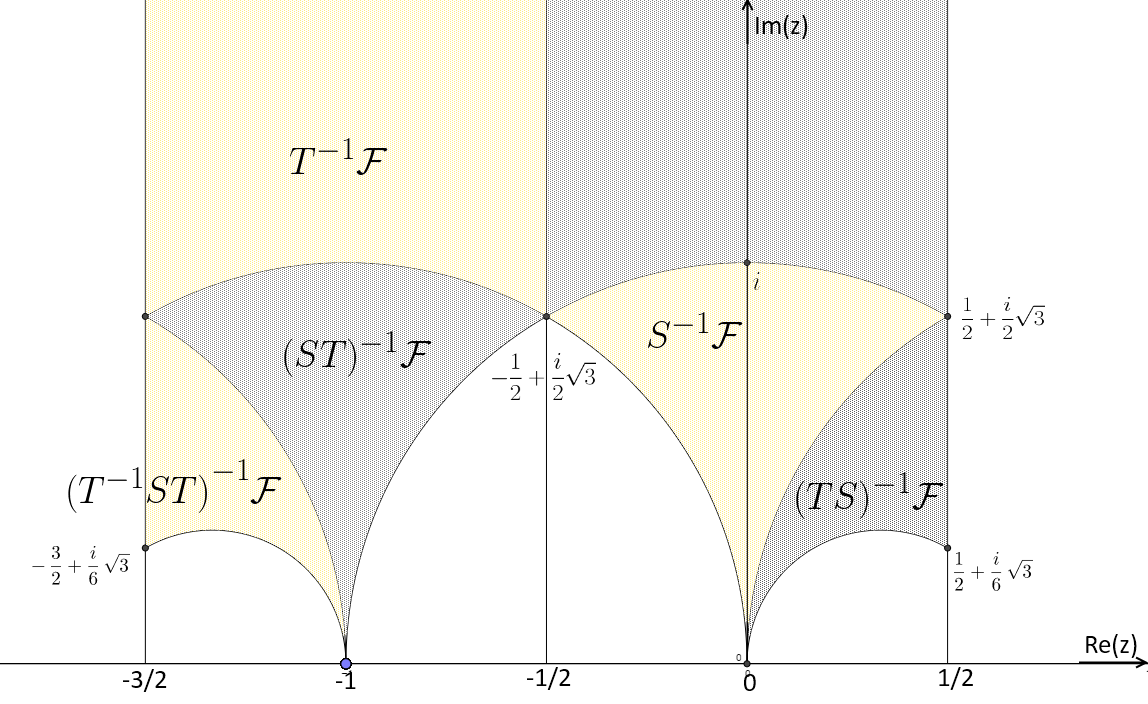
\includegraphics[height=3in]{FundamentalDomainGamma2}
    \else
      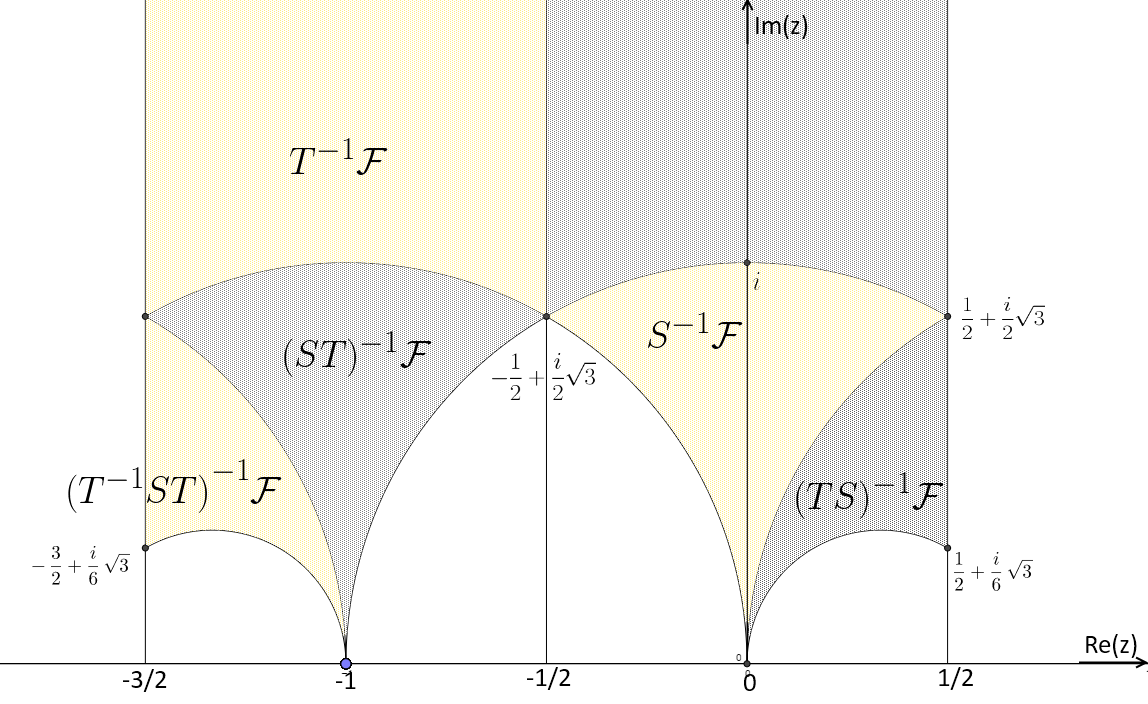
\includegraphics[bb = 92 86 545 742, height=6in]{FundamentalDomainGamma2}
    \fi
    \caption{Example: A Fundamental domain for $\Gamma(2)$}
    \label{fig:funDomainGammaTwo}
  \end{center}
\end{figure}


\end{example}

\begin{remark}
In \citep{verrill} an algorithm is described to construct fundamental domain's for certain congruence subgroups, like $\Gamma(N)$ and $\Gamma_0(N)$, so that the fundamental domain is connected and so that the triangles are "large" when drawn. The Java tool for drawing fundamental domains described in the paper is available at  http://www.math.lsu.edu/~verrill/fundomain/index2.html.
\end{remark}










